\section{Linked Environments for Atmospheric Discovery}
\label{se:lead}

\acrfull{lead} addresses the fundamental research challenges needed to create an integrated, scalable framework for adaptive analyzing and predicting the atmosphere \cite{Droegemeier2005Service-OrientedWeather}. To predict and analysis weather models by researchers, it required many resources. Rather than each researcher is running and handling own computer resources to do the weather experiments, \acrshort{lead} is providing pool of resources, then the researchers can use this resource pool to run their experiment in shorter amounts of time and in higher scale. At the time, researchers are developing their experiment flow, they are not using the resources many, and other are using it at the same time. LEAD's foundation is dynamic work flow orchestration and data management in a Web services framework \cite{Droegemeier2005Service-OrientedWeather}.

LEAD's complex array of services, applications, interfaces, and local and remote computing, networking, and storage resources is assembled by users in work flows to study mesoscale weather as it evolves \cite{Droegemeier2005Service-OrientedWeather}. As it follows the \acrshort{soa}, everything is implemented as independent services. This enable \acrshort{lead} to scale each service as required, and update each service without affecting other services. New models which are required for implementing a new forecast flow also has to be implement as a service and then integrate into the system.

Figure \ref{fi:lead_system} shows the fundamental capabilities of the \acrshort{lead} system. From the high-level view, \acrshort{lead} lets users query for and acquire information, simulate and predict weather by using numerical atmospheric models, assimilate data, analyze, mine, and visualize data and model output.

\begin{figure}[htp]
    \centering
    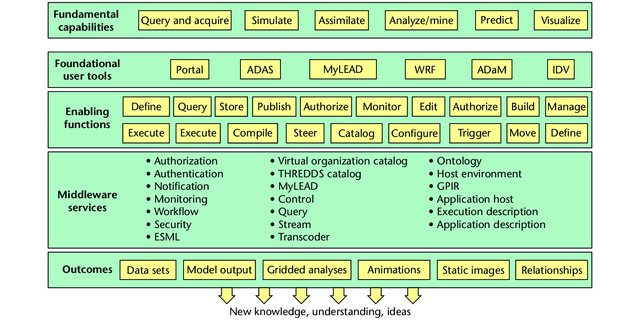
\includegraphics[width=1.0\textwidth]{lit/lead/LEAD-system-Fundamental-capabilities-familiar-to-meteorologists-are-shown-in-the-top_W640.jpg}
    \caption[Layered architecture of LEAD]{Layered architecture of LEAD \cite{Droegemeier2005Service-OrientedWeather}.}
    \label{fi:lead_system}
\end{figure}

\dbc{Fig. 2.4 should use full text width.}

The second level contains the fundamental tools that help to link services together. This include following tools \cite{Droegemeier2005Service-OrientedWeather};
\begin{itemize}
    \item a Web portal, the primary (though not exclusive) user entry point
    \item the ARPS Data Assimilation System (ADAS), a sophisticated tool for data quality control and assimilation
    \item myLEAD, a flexible metadata catalog service
    \item \acrfull{wrf} a next-generation atmospheric prediction and simulation model
    \item ADaM (Algorithm Development and Mining), a powerful suite of tools for mining observational data, assimilated data sets, and model output 
    \item Integrated Data Viewer (IDV) 
\end{itemize}

The Concept of the \acrshort{lead} is, the workflow orchestration for on-demand, real-time, dynamically adaptive systems, called as WOORDS. The system is doing the work flow orchestration as given in each procedure. Those procedural rules are define by researcher and feed into the system. The system is trying to perform the action immediate after the submission, and also it transmit the data, run the models and send back the put put with lower time delay as possible. According to the load and other requirement, the system will respond to those requirements automatically.

\begin{figure}[htp]
    \centering
    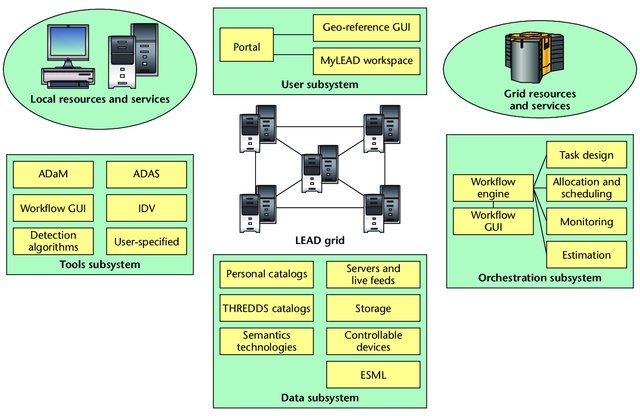
\includegraphics[width=1.0\textwidth]{lit/lead/LEAD-system-framework-LEAD-is-composed-of-several-interacting-subsystems-with-the-LEAD_W640.jpg}
    \caption[LEAD system framework]{LEAD system framework \cite{Droegemeier2005Service-OrientedWeather}.}
    \label{fi:lead_framework}
\end{figure}

As shown in the figure \ref{fi:lead_framework} LEAD consists of the following sub components, and it provides a distributed test bed for developing, integrating, and testing LEAD's components.
\begin{itemize}
    \item User subsystem -- comprises the LEAD portal and enable user can access services
    \item Data subsystem -- handles data and metadata, any numerical model output produced by operational or experimental models, and user generated information.
    \item Tools subsystem -- consists of all meteorological and IT tools
    \item Orchestration subsystem -- provides the technologies that let users manage data flows and model execution streams, and create and mine output. It also provides linkages to other software and processes for continuous or on-demand applications. 
\end{itemize}

\begin{figure}[htp]
    \centering
    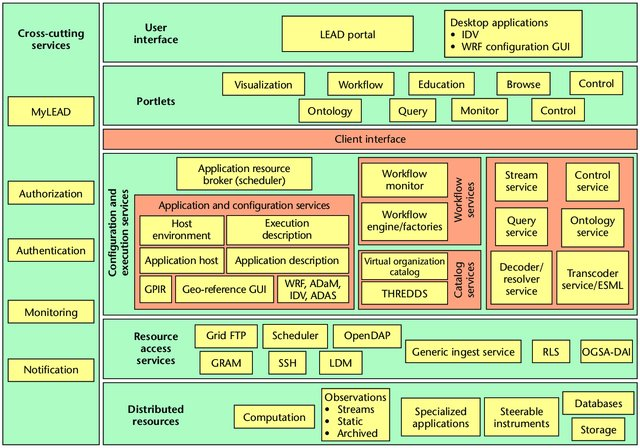
\includegraphics[width=1\textwidth]{lit/lead/LEADs-service-oriented-architecture-A-wide-variety-of-services-and-resources-grouped_W640.jpg}
    \caption[LEAD's service-oriented architecture]{LEAD's service-oriented architecture \cite{Droegemeier2005Service-OrientedWeather}.}
    \label{fi:lead_soa}
\end{figure}

\acrshort{soa}s are widely deployed in the commercial enterprise sector, and they form the foundation of many scientific "grid" technologies at the time of \acrshort{lead} design and developed. A variant of \acrshort{soa} is evolved later called as microservice architecture, and widely use in the industry nowadays.

As shown in figure \ref{fi:lead_soa}, \acrshort{lead} \acrshort{soa} has five distinct yet highly interconnected layers. 
The bottom layer represents raw computation, application, and data resources distributed throughout the LEAD grid and elsewhere. The next level up holds the Web services that provide access to raw services \cite{Droegemeier2005Service-OrientedWeather}. These two layers are working together, since \acrshort{lead} system resources are distributed over multiple locations and creating a pool of resources. The upper layer to the raw resources is abstracting the complexity of managing and accessing the resources, and provide a simplified access to the upper layer. In the Upper layers, it view as a unlimited resource pool for storing and handling data.

The configuration and execution services in the middle layer, consisting of five elements, represent services invoked by LEAD workflows. These are some critical aspects on a weather data management system. Most of the services listed here are required for creating work flows for weather data forecasting. Thus it is important to review them and understand the basic needs of a weather data management system.

\begin{itemize}
\item The application-oriented configuration service that manages the deployment and execution of real applications such as the \acrshort{wrf} simulation model, ADAS, and the ADaM tools \cite{Droegemeier2005Service-OrientedWeather}. When creating weather work flow, it is required to change the behaviour of model by changing some of the configurations of the model or run a different version of the model.
\item The application resource broker, which matches the appropriate host for execution to each application task, based on the execution’s time constraints \cite{Droegemeier2005Service-OrientedWeather}. This service is a critical part of the system, and responsible of using the resources of the system in optimized manner. When designing the weather data system, it is required to increase the capacity of the system automatically, and adopt into the system.
\item The workflow engine service, which drives experimental workflow instances, invokes both the configuration service and application resource broker \cite{Droegemeier2005Service-OrientedWeather}. This is a part of work flow orchestration.
\item The catalog services, represents the manner in which a user or application service discovers public-domain data products, or \acrshort{lead} services \cite{Droegemeier2005Service-OrientedWeather}. This is an important feature that should be available in a weather data system, and it is important to users to search for the availability of the data. Further wants to analyze the existing data for decision making.
\item Users require a host of data services to support rich query, access, and transformation operations on data products. An important goal behind LEAD is access transparency—facilitating user queries across all available heterogeneous data sources without adverse affects from different formats and naming schemes \cite{Droegemeier2005Service-OrientedWeather}. Users need to have transformation services to read data in different format. The query service gives the capability to search via available data without any affect on the data formats.
\end{itemize}
The top of the figure \ref{fi:lead_soa}, shows the user interface to the system. This give the access to individual services. When user logs into the system, based on the authentication and authorization setting bind to the individual account, the portlets can access the services on behalf of the user. Look into further details is not relevant to developing the \acrshort{wdias}, since the focus is not about workflow orchestration.

\acrshort{lead} is a more advanced system which can support for mesoscale weather prediction with the effort of multiple universities in the United State America with the effort of many of researchers and using many of computer resources. At the time it was building, it uses the \acrshort{soa} architecture as into its depth, and with the implementation each service can scale as needed and possible to enhance the service without interrupting other services. In the \acrshort{wdias} only focus on creating a framework that is extendable as system need more features as like \acrshort{lead} services.
